\geometry{paperwidth=200mm,paperheight=112.5mm}
\usepackage[utf8x]{inputenc}
\usepackage{amsmath,amsfonts,amssymb}
\usefonttheme{professionalfonts}
\usepackage{fontspec}
\setsansfont{URW Gothic}
\usecolortheme{default}
\usepackage{graphicx}
\usepackage{tikz}
\usepackage{hyperref}
\hypersetup{                                                                                                                                                                                                                   
  colorlinks = true,                                                                                                                                                                                                           
  urlcolor = MidnightBlue,                                                                                                                                                                                                     
  linkcolor = black                                                                                                                                                                                                            
}
\usepackage{caption}
\usepackage{nicefrac}
\usepackage{pifont}
\usepackage{minted}
\setminted{
  bgcolor = SkyBlue!15
}
%\usepackage{wrapfig}
%\usepackage{cutwin}
% for bkblock
\usepackage[most]{tcolorbox}

\usepackage[detect-none]{siunitx}
\sisetup{range-phrase = \text{--}}

\newcommand{\tr}{\operatorname{Tr}}
\newcommand{\re}{\operatorname{Re}}
\newcommand{\im}{\operatorname{Im}}
\newcommand{\C}{\mathbb{C}}
\newcommand{\R}{\mathbb{R}}
\newcommand{\ID}{\mathbb{I}}
\newcommand{\rf}{\mathcal{R}_5^{\mathbf{sp}}}
\newcommand{\hQpm}{\hat{Q}^{\pm}}
\newcommand{\hWpm}{\hat{W}^{\pm}}
\newcommand{\hQp}{\hat{Q}^{+}}
\newcommand{\hQm}{\hat{Q}^{-}}
\newcommand{\hWp}{\hat{W}^{+}}
\newcommand{\hWm}{\hat{W}^{-}}
\newcommand{\Wpm}{W^{\pm}}
\newcommand{\Qpm}{Q^{\pm}}
\newcommand{\Qp}{Q^{+}}
\newcommand{\Qm}{Q^{-}}
\newcommand{\Wp}{W^{+}}
\newcommand{\Wm}{W^{-}}
\newcommand{\Qnd}{Q_{\textrm{ND}}}
\newcommand{\Tee}{T_{ee}}
\newcommand{\Too}{T_{oo}}
\newcommand{\Moe}{M_{oe}}
\newcommand{\Moo}{M_{oo}}
\newcommand{\Meo}{M_{eo}}
\newcommand{\Mee}{M_{ee}}
\newcommand{\order}{\mathcal{O}}

\newcommand{\Sg}{S_\mathrm{G}}
\newcommand{\Sdeg}{S_\mathrm{deg}}
\newcommand{\Smusig}{S_{\mu_\sigma}}
\newcommand{\Sdel}{S_\delta}
\newcommand{\mudel}{\mu_\delta}
\newcommand{\musig}{\mu_\sigma}
\newcommand{\mutilsig}{\tilde{\mu}_\sigma}
\newcommand{\mutildel}{\tilde{\mu}_\delta}
\newcommand{\mul}{\mu_\ell}
\newcommand{\D}{\mathcal{D}}
\newcommand{\dtau}{\delta\tau}

\newcommand{\csw}{c_\mathrm{sw}}
\newcommand{\mpcac}{m_\mathrm{PCAC}}
\newcommand{\Ntraj}{N_\mathrm{traj}}
\newcommand{\Nmeas}{N_\mathrm{meas}}
\newcommand{\Nconf}{N_\mathrm{conf}}
\newcommand{\Mpi}{M_{\pi^\pm}}
\newcommand{\Mphyspi}{M_{\pi^\pm}^\mathrm{phys}}
\newcommand{\Fpi}{f_{\pi^\pm}}
\newcommand{\Mpin}{M_{\pi^0}}
\newcommand{\Mpinc}{M_{\pi^{(0,c)}}}
\newcommand{\ld}{\mathrm{(LD)}}
\newcommand{\cd}{\mathrm{(CD)}}

\newcommand{\fnabla}{\nabla^\mathrm{f}}
\newcommand{\bnabla}{\nabla^\mathrm{b}}

\newcommand{\mps}{M_\mathrm{P}}
\newcommand{\ps}{\mathrm{P}}
\newcommand{\mpi}{M_\pi}
\newcommand{\mphyspi}{M_{\pi}^\mathrm{phys}}
\newcommand{\fps}{f_\mathrm{P}}
\newcommand{\fpi}{f_\pi}
\newcommand{\mcrit}{m_\mathrm{crit}}
\newcommand{\mw}{m_\mathrm{W}}
\newcommand{\kc}{\kappa_c}
\newcommand{\mn}{M_\mathrm{N}}
\newcommand{\dof}{\mathrm{dof}}

\newcommand{\lmin}{\lambda_\mathrm{min}}
\newcommand{\lmax}{\lambda_\mathrm{max}}
\newcommand{\qcdlambda}{\Lambda_\mathrm{QCD}}

\newcommand{\chipt}{$\chi$PT}
\newcommand{\wchipt}{W$\chi$PT}
\newcommand{\wtmchipt}{Wtm$\chi$PT}

\newcommand{\dingcircle}{\ding{108}}
\newcommand{\dingsquare}{\ding{110}}
\newcommand{\dingtriangle}{\ding{115}}

\newcommand{\mev}{~\mathrm{MeV}}
\newcommand{\gev}{~\mathrm{GeV}}
\newcommand{\fm}{~\mathrm{fm}}

\newcommand{\nmev}{\mathrm{MeV}}
\newcommand{\ngev}{\mathrm{GeV}}
\newcommand{\nfm}{\mathrm{fm}}

\newcommand{\Fav}{\|F\|_\mathrm{av}^2}
\newcommand{\Fmax}{\|F\|_\mathrm{max}^2}
\newcommand{\Fsq}{\|F\|^2}
\newcommand{\mutil}{\tilde{\mu}}
\newcommand{\rhotil}{\tilde{\rho}}
\newcommand{\ctil}{\tilde{c}_\mathrm{sw}}

% full page width float
%   \checkoddpage
%   \edef\side{\ifoddpage l\else r\fi}%
%   \makebox[\textwidth][\side]{%
%   \begin{minipage}{1.35\linewidth}
%   \end{minipage}
%   }%

% margin figure
% \marginpar{
%   \centering
%   \includegraphics[width=\linewidth]{}
%   \captionof{figure}[]{}
%   \label{}
% }

\newtcolorbox{bkblock}[2][]{%
  left=0pt,
  right=0pt,
  top=0pt,
  bottom=0pt,
  colback=bg,
  colframe=structure!100,
  fonttitle=\sffamily,
  coltitle=structure!100,
  colbacktitle=structure!10,
  enhanced,
%  attach boxed title to top left={yshift=-0.5mm, xshift=1mm},
  title=#2,
  #1}

\newtcolorbox{bkexampleblock}[2][]{%
  left=0pt,
  right=0pt,
  top=0pt,
  bottom=0pt,
  colback=bg,
  colframe=example text.fg!100,
  fonttitle=\sffamily,
  coltitle=example text.fg!100,
  colbacktitle=example text.fg!10,
  enhanced,
%  attach boxed title to top left={yshift=-0.5mm, xshift=1mm},
  title=#2,
  #1}

\newtcolorbox{bkalertblock}[2][]{%
  left=0pt,
  right=0pt,
  top=0pt,
  bottom=0pt,
  colback=bg,
  colframe=alert!100,
  fonttitle=\sffamily,
  coltitle=alert!100,
  colbacktitle=alert!10,
  enhanced,
%  attach boxed title to top left={yshift=-0.5mm, xshift=1mm},
  title=#2,
  #1}



%compact itemize, perfect for talks
\setlength{\leftmargin}{0pt}
\setlength{\leftmargini}{0.4cm}
\setlength{\leftmarginii}{0.2cm}

\usefonttheme{professionalfonts} 

\newcommand{\roundbox}[1]{%
\noindent\begin{tikzpicture}%
  \draw node[draw=lightgray,fill=white,rounded corners,inner sep=1ex] {%
  #1
  };%
\end{tikzpicture}%
}%

\definecolor{DarkBlue}{HTML}{002e77}
\definecolor{LightBlue}{HTML}{6495ed}
\definecolor{MidGreen}{HTML}{228b22}
\definecolor{DarkGreen}{HTML}{006400}
\definecolor{HotPink}{HTML}{dc143c}
\definecolor{LightPeach}{HTML}{ff7f50}
\definecolor{LightOrange}{HTML}{ffa500}
\definecolor{LighterOrange}{HTML}{ffcf9d}    
\definecolor{RedBrown}{HTML}{8b3e2f}
\definecolor{DarkRed}{HTML}{8b3e2f}

\usetheme{Boadilla}
\usecolortheme[named=DarkBlue]{structure}
\useinnertheme{rounded}

\setbeamertemplate{navigation symbols}{}

\graphicspath{{graphics/}}

\title[Kronos]{Kronos : A lattice QCD library accelerated with Kokkos}
\author[A. Sen, B. Kostrzewa]{Aniket Sen, Bartosz Kostrzewa  \\ \vspace{0.2cm} in collaboration with \\ \vspace{0.2cm} \centering Travis Whyte, Eric Gregory, Stefan Krieg, Giovanni Pederiva, Simon Schlepphorst}
\institute[HISKP]{HISKP \& FZJ}
\titlegraphic{\roundbox{
\includegraphics[height=2.4cm]{graphics/uni_bonn_hiskp_FZJ_numeriqs_ETMC}}}
\date[ETMC meeting 2025]{\small ETMC meeting 2025, 28.08.2025}
\subject{subject}
\keywords{keywords}


\begin{document}

\begin{frame}
  \titlepage{}
\end{frame}

% \begin{frame}{Technical Overview}
%   Test
% \end{frame}

\begin{frame}{Motivation}
  \begin{itemize}
    \item Lattice QCD code for the next generation of exascale clusters
  \end{itemize} 
  \vspace{0.5cm}
  Key features: \\
  \begin{itemize}
    \item Performance portable : single architecture agnostic codebase
    \item Easy to use : reduce entry barrier for new users
  \end{itemize}


  AS: Bartek please make this slide more interesting
\end{frame}

\begin{frame}{CPUs vs GPUs}
  \centering
  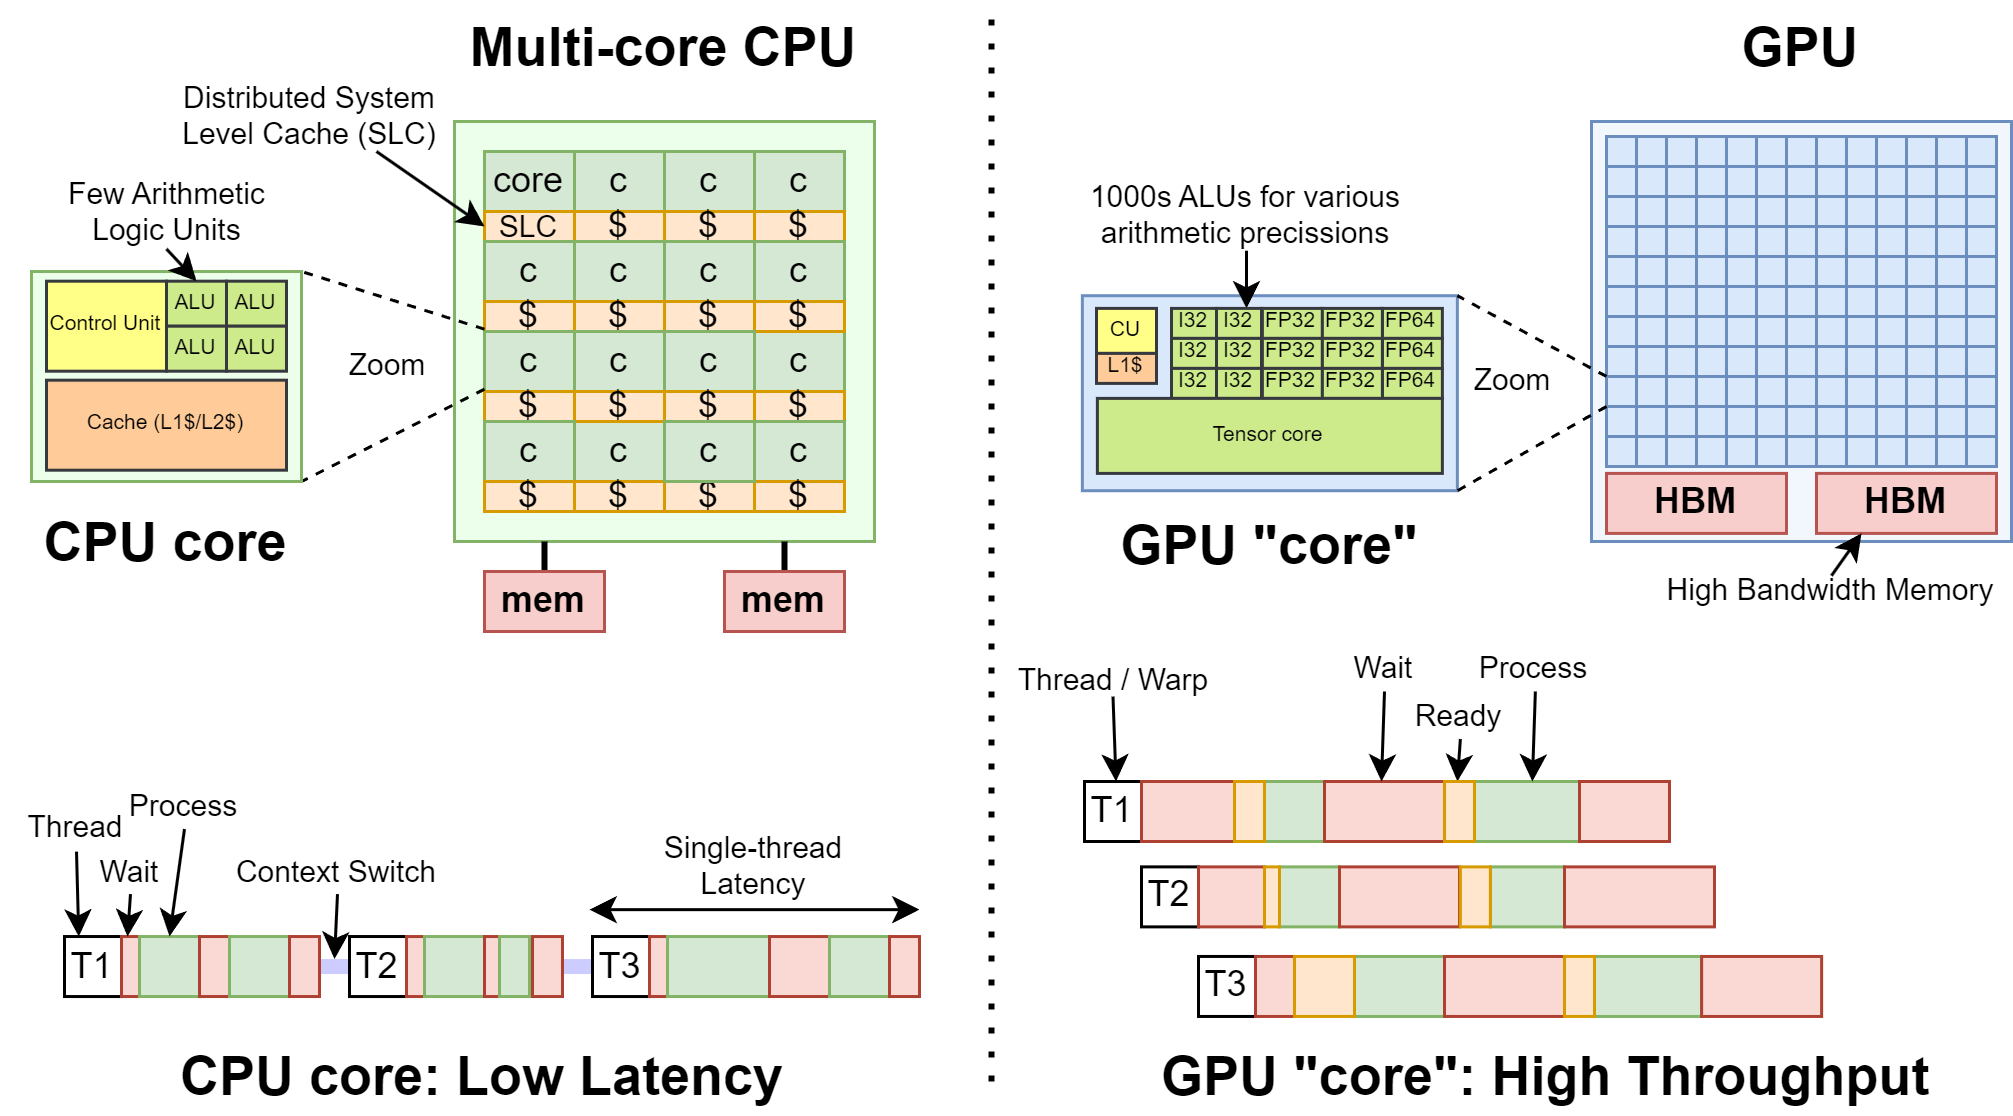
\includegraphics[height=0.8\paperheight]{graphics/cpuVSgpu.png}\\
  \footnotesize{\href{https://www.frontiersin.org/journals/physics/articles/10.3389/fphy.2025.1542474/full}{[E.~Suarez, J.~Amaya, O.~Freyermuth, M.~Girone, \textbf{BK}, S.~Pfalzner, \emph{Energy efficiency trends in HPC: what high-energy and astrophycisists need to know}, Front.in Phys. 13 (2025) 1542474]}}
\end{frame}                                                    

\begin{frame}{Data Layout Matters}
  \begin{itemize}
    \item Consider an $8 \times 8$ lattice of scalar values.
    \vspace{0.1cm}
    \item Could lay out in memory as \mintinline{c++}{real[y][x]}, or when linearised, \mintinline{c++}{real[i]}, where \mintinline{c++}{i} $\in [0,63]$.
    \vspace{0.1cm}
    \item Iterate over this on CPU and GPU in some kind of \mintinline{c++}{parallel for}, spltting the work across the available threads.
  \end{itemize}
  \begin{columns}
    \column{0.5\linewidth}
      \only<1>{
        \begin{center}
          
\includegraphics[height=0.6\paperheight]{graphics/grid}
        \end{center}
      }
      \only<2>{
        \begin{center}
          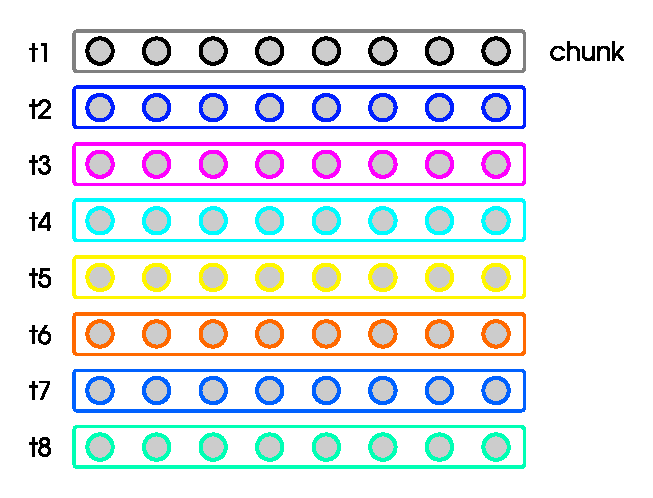
\includegraphics[height=0.6\paperheight]{graphics/grid_cpu}
        \end{center}
      }
      \only<3>{
        \begin{itemize}
          \item On GPU, threads are unit of vectorisation AND parallelisation.
          \vspace{0.6cm}
          \item Work is scheduled in blocks which must (ideally) be multiple of \emph{team} size.
            \begin{itemize}
              \item NVIDIA $\rightarrow$ team = warp, size 32
              \item AMD $\rightarrow$ team = wavefront, size 64
            \end{itemize}
          \vspace{0.6cm}
          \item Threads within team should access neighbouring memory locations (\emph{coalesced access}).
          \begin{itemize}
            \item Performance loss factor up to $\approx 100$ if not done! 
          \end{itemize}
        \end{itemize}
      }
    \column{0.5\linewidth}
      \only<2>{
        \begin{itemize}
          \item On CPU, ideally each thread (tX) processes a chunk of contiguous memory.
          \vspace{0.6cm}
          \item Threads operate on chunks of memory as far apart as possible.
          \vspace{0.6cm}
          \item If possible, compiler exploits SIMD unit to process multiple values in parallel per clock cycle.
          \begin{itemize}
            \item For problems with low arithmetic intensity (like lattice QCD), loss factor small if SIMD not optimally used.
          \end{itemize}
        \end{itemize}
      }
      \only<3>{
        \begin{center}
          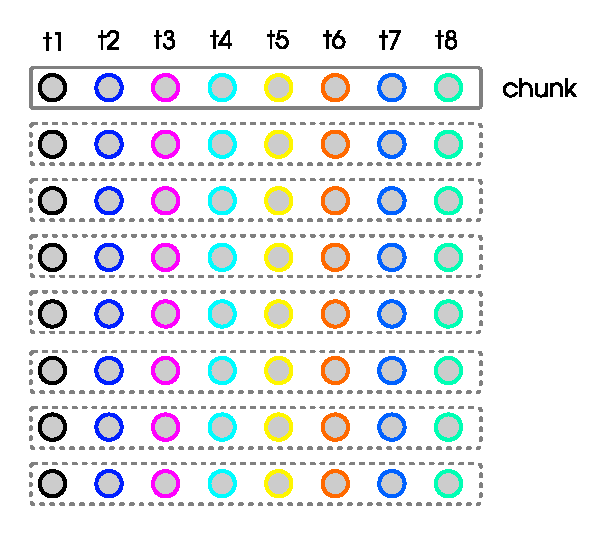
\includegraphics[height=0.65\paperheight]{graphics/grid_gpu}
        \end{center}
      }
  \end{columns}
\end{frame}

\begin{frame}{Data Layout Matters}
  \begin{columns}
    \column{0.5\linewidth}
      \begin{center}
        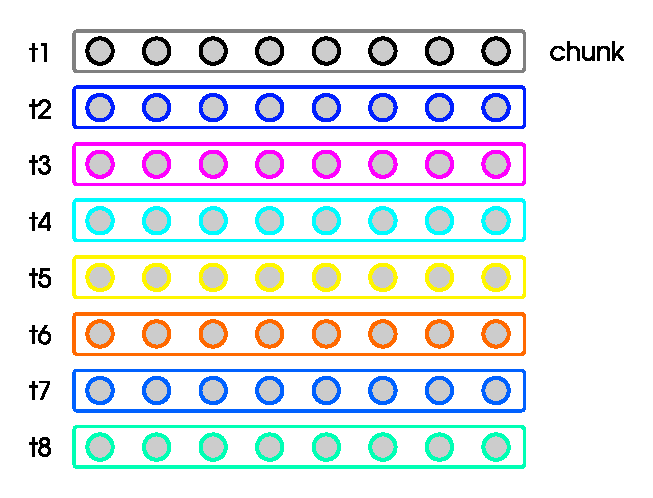
\includegraphics[height=0.6\paperheight]{graphics/grid_cpu}
      \end{center}
    \column{0.5\linewidth}
      \begin{center}
        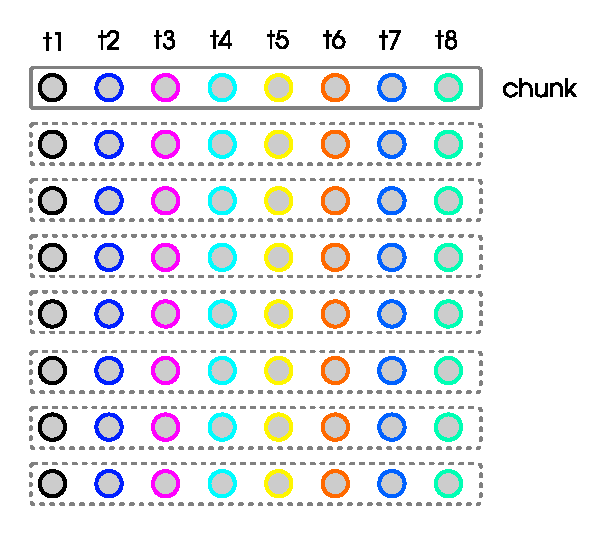
\includegraphics[height=0.65\paperheight]{graphics/grid_gpu}
      \end{center}
  \end{columns}
  \begin{itemize}
    \item Without internal structure this is more or less trivial.
  \end{itemize}
\end{frame}

\begin{frame}{Data Layout Matters}
  \begin{columns}
    \column{0.45\linewidth}
      \begin{center}
        \includegraphics[width=0.85\linewidth]{graphics/grid_su3_spinor}
      \end{center}
    \column{0.5\linewidth}
      \begin{itemize}
        \item<1-> $U^{ab}_\mu(x) \rightarrow$ \mintinline{c++}{complex[x][mu][a][b]}
        \vspace{0.2cm}
        \item<1-> $\psi^{\sigma b}(x) \rightarrow$ \mintinline{c++}{complex[x][sigma][b]}
        \vspace{0.2cm}
        \begin{itemize}
          \item Consecutive lattice sites $x$ separated by e.g. \mintinline{c++}{4 * sizeof(su3)} or \mintinline{c++}{sizeof(spinor)} in memory.
        \end{itemize}
        \vspace{0.6cm}
        \item<3-> \emph{Array of Struct} layout works well on \textbf{CPU} due to cache hierarchy and small SIMD loss factor.
        \vspace{0.6cm}
        \item<4-> On \textbf{GPU} would like to have $x$ running fastest:
        \vspace{0.2cm}
        \begin{itemize}
          \item \emph{Struct of Array} layout.
          \vspace{0.3cm}
          \item In C notation: $\psi(x)^{\sigma b} \rightarrow$ \mintinline{c++}{complex[b][sigma][x]}
        \end{itemize}
      \end{itemize}
  \end{columns}
  \vspace{0.4cm}
  \begin{itemize}
    \item<5-> Grid: virtual node vectorisation (site fusion) $\rightarrow$ SIMD length = multiple of thread team size
    \begin{itemize}
      \item same (complicated) layout gives very good performance on CPU and GPU, but need to pack / unpack
    \end{itemize}
    \vspace{0.4cm}
    \item<6-> Alernative: \textbf{switch memory order of indices when switching from CPU to GPU}
    \begin{itemize}
      \item generally obtain reasonably good performance on both 
    \end{itemize}
  \end{itemize}
\end{frame}

\begin{frame}{Slicing Multi-dimensional Iteration Spaces}
  \only<1>{
    \begin{center}
      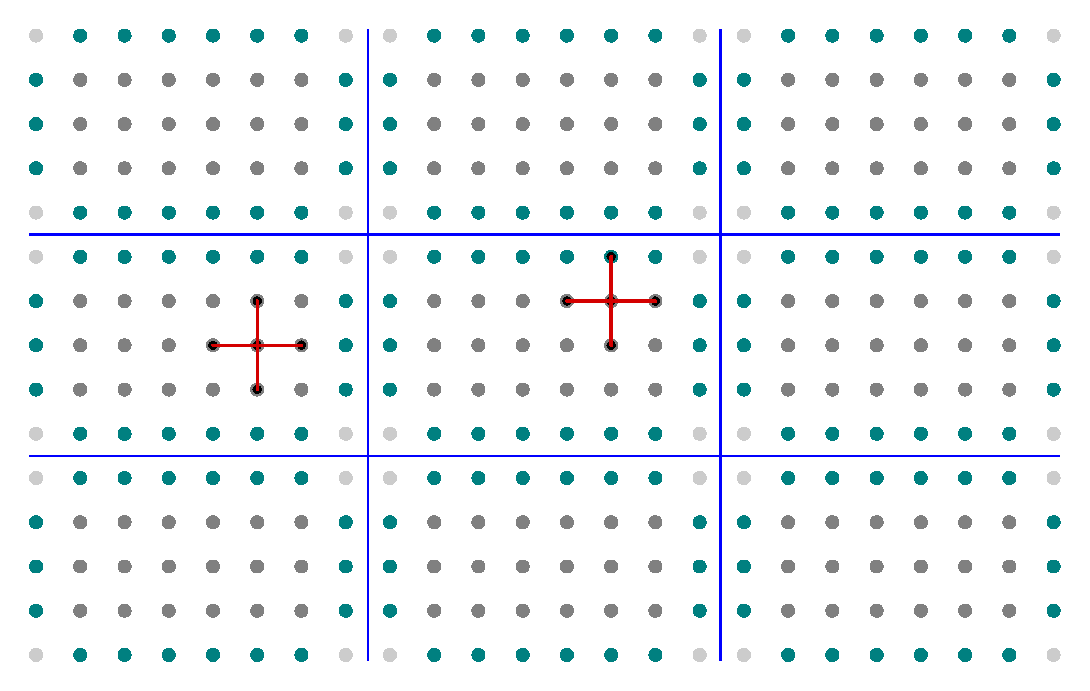
\includegraphics[height=0.75\paperheight]{graphics/regular_mesh_halo_exchange_2c}\\
      \textbf{Let's try to overlap communication and computation for a next-neighbour stencil.}
    \end{center}
  }  
  \only<2>{
    \begin{center}
      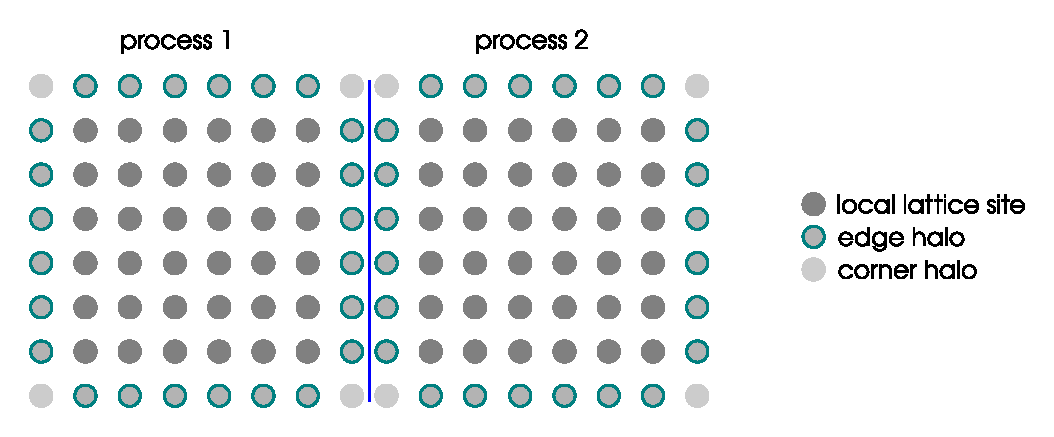
\includegraphics[height=0.7\pageheight]{graphics/halo_exchange_algo_1}\\
      \textbf{Domain-decompose a 2D lattice and allocate a halo of depth 1.}
    \end{center}
  }
  \only<3>{
    \begin{center}
      \includegraphics[height=0.75\pageheight]{graphics/halo_exchange_algo_2}\\
      \textbf{Start non-blocking communication.}
    \end{center}
  }
  \only<4>{
    \begin{center}
      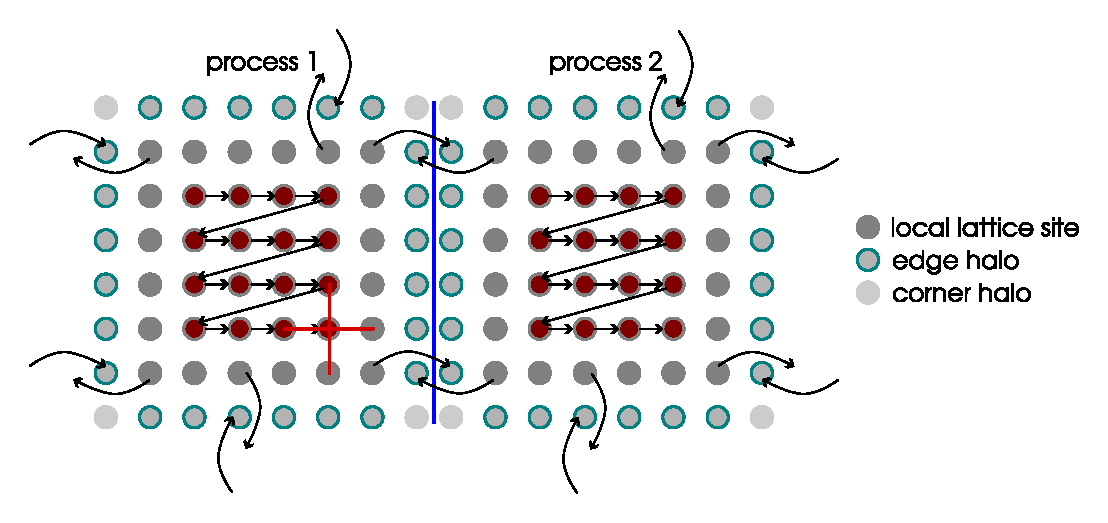
\includegraphics[height=0.75\pageheight]{graphics/halo_exchange_algo_3}\\
      \textbf{Apply stencil on interior (bulk) of the volume:} $\rightarrow$ \mintinline{c++}{x, y} $\in [1,N_{x,y}-2]$
    \end{center}
  }
  \only<5>{
    \begin{center}
      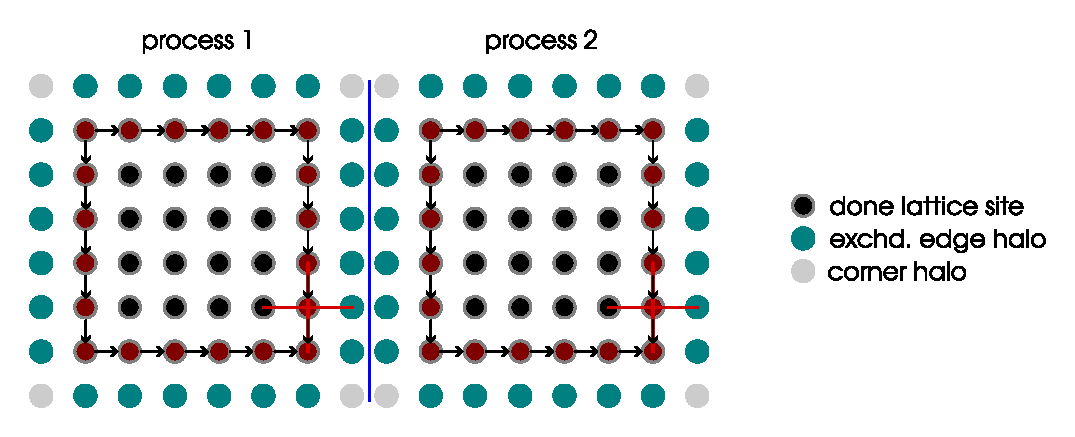
\includegraphics[height=0.7\pageheight]{graphics/halo_exchange_algo_4}\\
      \vspace{0.3cm}
      \begin{columns} 
        \column{0.4\linewidth}
          \hfill \textbf{Apply stencil on surface:}
        \column{0.6\linewidth}
          $\rightarrow$ \mintinline{c++}{x} $\in 0,N_x-1$; \mintinline{c++}{y} $\in [0,N_y-1]$\\
          $\rightarrow$ \mintinline{c++}{y} $\in 0,N_y-1$; \mintinline{c++}{x} $\in [1,N_x-2]$
      \end{columns}
    \end{center}
  }
\end{frame}

\begin{frame}[fragile]{Slicing Multi-dimensional Iteration Spaces}{API}
    \begin{itemize}
      \item<1-> Would like to have a parallel launch mechanism which can easily run over slices of the multi-dimensional iteration space, for example in 4D.
      \vspace{0.6cm}
    \item<2-> For bulk:\\ 
      \begin{minted}{c++}
  int begin[4] = {1,1,1,1};
  int end[4] = {N1-1,N2-1,N3-1,N4-1}; 
  parallel_for(begin,end,stencil); // iterates over 1 to Nx-2
      \end{minted}
      \item<3-> For surfaces, e.g. in +3 direction: 
      \begin{minted}{c++}
  int begin[4] = {0,0,N3-1,0};
  int end[4] = {N1,N2,N3,N4};
  parallel_for(begin,end,stencil);
      \end{minted}
      \vspace{-0.5cm}
      \begin{itemize}
        \item Loop over the 8 directions: surface kernel launched as soon as respective comms is completed.
      \end{itemize}
      \vspace{0.6cm}
      \item<4-> \textbf{Launch mechanism must map iteration space well to CPU threads and blocks of GPU thread teams.}
    \end{itemize}
\end{frame}

\begin{frame}{Kokkos}
  The Kokkos C++ Performance Portability Ecosystem is a production
  level solution for writing modern C++ applications in a hardware agnostic way.\\
  
  \begin{bkblock}{Supported HPC architectures:}
    \begin{itemize}
      \item CUDA
      \item HIP
      \item SYCL
      \item HPX
      \item OpenMP
    \end{itemize}
  \end{bkblock}

  Based on concepts of:
  \begin{itemize}
    \item execution : execution space, execution pattern, execution policy
    \item memory: memory space, memory layout, memory trait
  \end{itemize}
\end{frame}

\begin{frame}[fragile]{Kokkos : Memory}{Views}
  \begin{minted}{c++}
template <class DataType [, class LayoutType] [, class MemorySpace] [, class MemoryTraits]>
class View;
  \end{minted}
  \begin{itemize}
    \item \verb|DataType| : defines the fundamental scalar type of the \verb|View| and its dimensionality
    \item \verb|LayoutType| : mapping of the indices onto the underlying 1D memory storage (\verb|LayoutRight|, \verb|LayoutLeft|)
    \item \verb|MemorySpace| : storage location of the view (device/host, related to the execution space)
    \item \verb|MemoryTraits| : access properties (\verb|Unmanaged|, \verb|RandomAccess|, ...)
  \end{itemize}

  example:
  \begin{minted}{c++}
# default layout of the execution space
using ViewLayout = Kokkos::DefaultExecutionSpace::array_layout;
# memory space of the execution space
using ViewSpace  = Kokkos::DefaultExecutionSpace::memory_space;
# a 2D view of ints with 2 dynamic extents
Kokkos::View<int**, ViewLayout, ViewSpace> a("a", 10, 12);
# a 3D view of doubles with 1 dynamic and 2 compiled extents
Kokkos::View<double*[4][3], ViewLayout, ViewSpace> b("b", 16);
  \end{minted}
\end{frame}

\begin{frame}[fragile]{Kokkos : Execution}{Policy}
  Kokkos abstracts the execution policy via

  \begin{columns}
    \column{0.4\textwidth}
      \begin{block}{RangePolicy}
        defines an execution policy for a 1D iteration space
      \end{block}
      \begin{minted}{c++}
Kokkos::RangePolicy(
  execution_space, 
  begin, end, 
  chunk_size);
      \end{minted}
    \column{0.4\textwidth}
      \begin{block}{MDRangePolcy}
        defines an execution policy for a multidimensional iteration space
      \end{block}
      \begin{minted}{c++}
Kokkos::MDRangePolicy<
  Kokkos::Rank<N>>(
    execution_space, 
    begin, end, 
    tiling);
  \end{minted}
  \end{columns}

  \begin{bkblock}{Parameters:}
    \begin{itemize}
      \item The iteration space starts at \verb|begin| and goes to \verb|end| with open interval.
      \item \verb|Rank<N>| determines the dimensionality of the multidimensional iteration space.
      \item The block sizes are controlled by \verb|chunk_size| and \verb|tiling|.
    \end{itemize}
  \end{bkblock}
\end{frame}

\begin{frame}[fragile]{Kokkos : Execution}{Parallel Dispatches}
  Kokkos executes kernels via the parallel dispatches

  \begin{itemize}
    \item \verb|parallel_for| : implements a “for loop” with independent iterations.
    \item \verb|parallel_reduce| : implements a reduction.
    \item \verb|parallel_scan| : implements a prefix scan.
  \end{itemize}

  \begin{columns}
    \column{0.45\textwidth}
      parallel\_for:
      \begin{minted}{c++}
template<
  class ExecPolicy, 
  class FunctorType>
Kokkos::parallel_for(
  const std::string &name, 
  const ExecPolicy &policy, 
  const FunctorType &functor);
      \end{minted}
    \column{0.45\textwidth}
    parallel\_reduce:
    \begin{minted}{c++}
template <
  class ExecPolicy, 
  class FunctorType, 
  class... ReducerArgument>
Kokkos::parallel_reduce(
  const std::string& name,
  const ExecPolicy& policy,
  const FunctorType& functor,
  const ReducerArgument&... reducer);
    \end{minted}
  \end{columns}
\end{frame}

\begin{frame}[fragile]{A simple kernel with Kokkos}{parallel\_for}
  \begin{columns}
    \column{0.55\textwidth}
      \begin{minted}{c++}
const int N = 16;
Kokkos::View<double*> a("a", N);
Kokkos::deep_copy(a, 2.0);
Kokkos::View<double*> b("b", N);
Kokkos::deep_copy(b, 3.0);
Kokkos::View<double*> c("c", N);
auto policy = Kokkos::RangePolicy(0, N);
Kokkos::parallel_for(
  "add",
  policy,
  KOKKOS_LAMBDA(int i) {
    c(i) = a(i) + b(i)
  }
);
Kokkos::fence();
      \end{minted}
    \column{0.4\textwidth}
      \begin{block}{c = a + b}
        \begin{itemize}
          \item initialize the 1D views
          \item \verb|deep_copy| copies the single scalar value to every site in the view
          \item Kokkos views are accessed via \verb|operator()(indices...)|
          \item the functor can be a lambda
          \item \verb|fence()| creates a barrier in the execution space
        \end{itemize}
      \end{block}
  \end{columns}
\end{frame}

\begin{frame}[fragile]{A simple kernel with Kokkos}{parallel\_reduce}
  \begin{columns}
    \column{0.55\textwidth}
      \begin{minted}{c++}
const int N1 = 16;
const int N2 = 12;
Kokkos::View<double**> a("a", N1, N2);
Kokkos::deep_copy(a, 5.0);
double sum = 0;
auto policy = Kokkos::MDRangePolicy<
                Kokkos::Rank<2>>(
                  {0, 0}, {N1, N2}
                );
Kokkos::parallel_reduce(
  "reduce_sum",
  policy,
  KOKKOS_LAMBDA(int i, int j, 
    double &lsum) {
      lsum += a(i, j);
    },
  Kokkos::Sum<double>(sum)
);
Kokkos::fence();
      \end{minted}
    \column{0.4\textwidth}
      \begin{block}{sum over a 2D view}
        \begin{itemize}
          \item similar to \verb|parallel_for|
          \item needs a local reduction variable along with the policy iteration indices
        \end{itemize}
      \end{block}
    \end{columns}
\end{frame}

\begin{frame}[fragile]{A more general kernel using functors}
  A more generalized addition kernel for different dimensionality and site types
  \begin{columns}
    \column{0.6\textwidth}
      \begin{minted}{c++}
template <typename view_t>
struct add {
  const view_t m_a;
  const view_t m_b;
  view_t m_c;

  add(view_t &c, const view_t &a, const view_t &b) :
    m_a(a), m_b(b), m_c(c) {}
  
  template <typename... IndexTypes>
  KOKKOS_INLINE_FUNCTION
  void operator()(IndexTypes... indices) const noexcept
  {
    m_c(indices...) = m_a(indices...) + m_b(indices...)
  }
};
      \end{minted}
    \column{0.38\textwidth}
      \begin{minted}{c++}
const int N = 12;
using view_t = Kokkos::View<int*>;
view_t a("a", N);
view_t b("b", N);
view_t c("c", N);
auto add_func = add(c, a, b);
auto policy = Kokkos::RangePolicy(
                0, N
              );
Kokkos::parallel_for(
  "add_functor",
  policy,
  add_func
);
Kokkos::fence();
      \end{minted}
  \end{columns}

  This works as long as the "+" and "=" operators for the intrinsic site type is well defined
\end{frame}

\begin{frame}[fragile]{Kronos: Site types}
  To use Kokkos views as lattice fields, it is useful to define our own site types.\\

  For example
  \begin{block}{ColourMatrix}
    Complex valued $SU(N)$ matrix\\
    we can use Kokkos Array structure to
    store the matrix
  \end{block}


  \begin{minted}{c++}
template <typename RT, idx_t Ncol>
struct ColourMatrix : public Array<Array<cplx_t<RT>, size_t(Ncol)>, size_t(Ncol)>;
  \end{minted}
  
  And define an accessor \verb|elem| as

  \begin{minted}{c++}
KOKKOS_FORCEINLINE_FUNCTION
const auto &
elem(idx_t c1, idx_t c2) const noexcept
{
  return (*this)[c1][c2];
}
  \end{minted}

\end{frame}

\begin{frame}[fragile]{Kronos: Field structure}{ScalarField}
  we define wrapper classes around the Kokkos Views to
  define fields on the lattice\\

  \begin{block}{ScalarField}
    A single site type object resides at
    every lattice site
  \end{block}

  \begin{minted}{c++}
template <ValidSiteType SiteType, typename Layout,
  idx_t Ndim, typename MemorySpace 
    = Kokkos::DefaultExecutionSpace::memory_space>
class ScalarField;
  \end{minted}

  \begin{itemize}
    \item the dynamic extent corresponds to the lattice sites in a lexicographic ordering
    \item \verb|Ndim| defines the dimensionality of the lattice
  \end{itemize}

  example:

  \begin{minted}{c++}
template <typename RT, idx_t Ns, idx_t Nc>
using SpinorField4D = ScalarField<Spinor<RT, Ns, Nc>, cplx_t<RT> *[Ns][Nc], 4>;
  \end{minted}

\end{frame}

\begin{frame}[fragile]{Kronos: Field structure}{VectorField}
  we define wrapper classes around the Kokkos Views to
  define fields on the lattice\\

  \begin{block}{VectorField}
    A vector of site type object at
    every lattice site
  \end{block}

  \begin{minted}{c++}
template <ValidSiteType SiteType, typename Layout,
  idx_t Ndim, idx_t Vdim,
  typename MemorySpace 
    = Kokkos::DefaultExecutionSpace::memory_space>
class VectorField;
  \end{minted}

  \begin{itemize}
    \item \verb|Vdim| defines the length of the vector at each site
  \end{itemize}

  example:

  \begin{minted}{c++}
template <typename RT, idx_t Nc>
using GaugeField4D = VectorField<ColourMatrix<RT, Nc>, cplx_t<RT> *[4][Nc][Nc], 4, 4>;
  \end{minted}

\end{frame}

\begin{frame}[fragile]{Kronos: Site reference}
  
  \begin{bkalertblock}{How do we extract the site type structure from the View without copies?}
    use a reference wrapper
  \end{bkalertblock}

  For example, in the case of the gauge field, we define a
  \verb|SiteGaugeLink| reference

  \begin{minted}{c++}
template <ValidGaugeFieldType gauge_t, idx_t Ncol>
class SiteGaugeLink {
 private:
  idx_t m_i;
  idx_t m_mu;
  const gauge_t &m_f;
}
  \end{minted}

  which accesses the $SU(N)$ matrix for the gauge field \verb|m_f| at lattice index
  \verb|m_i| and vector index \verb|m_mu|\\

  Accordingly, the accessor \verb|elem| takes the form

  \begin{minted}{c++}
KOKKOS_FORCEINLINE_FUNCTION
auto &
elem(idx_t c1, idx_t c2) const noexcept
{
  return m_f(m_i, m_mu, c1, c2);
}
  \end{minted}

\end{frame}

\begin{frame}[fragile]{Kronos: Concepts}

  \begin{bkalertblock}{How do we ensure correct combination of site types and field types in different operators and functions?}
    use concepts (since C++20)
  \end{bkalertblock}

  For example, a valid colourmatrix type must satisfy the following

  \begin{minted}{c++}
template <typename T>
concept ValidColourMatrixType = requires {
  typename T::is_colour_matrix;                          // unambiguous type trait
  typename T::value_type;                                // type of matrix elements
  typename T::real_t;                                    // which (float point) type
  requires std::is_same_v<decltype(T::Nc), const idx_t>; // number of colours
} && requires(T t) { 
    t.elem(std::declval<int>(), std::declval<int>()); 
  }; // an elem() to access the matrix elements
  \end{minted}

\end{frame}

\begin{frame}[fragile]{Kronos: Opeator overloads on site types}

  we can define operator overloads between site types.\\

  For example a product of colourmatrix and spinor can be defined as

  \begin{minted}{c++}
template <
  ValidColourMatrixType LHS,
  ValidSpinorType RHS,
  typename std::enable_if_t<LHS::Nc == RHS::Nc, int> = 0>
KOKKOS_FORCEINLINE_FUNCTION auto
operator*(const LHS &lhs, const RHS &rhs) noexcept { ... }
  \end{minted}

  this works for any combination of actual site types and reference types

\end{frame}

\begin{frame}[fragile]{Kronos: A simple kernel}

  we can write a simple kernel to add two Spinor fields as\\

  \begin{minted}{c++}
template <ValidSpinorFieldType spinor_t>
void add_spinor(spinor_t &c, const spinor_t &a, const spinor_t &b) {
  Kokkos::parallel_for("add_spinor", a.m_n,
    KOKKOS_LAMBDA(idx_t i) {
      auto A = a.site(i);
      auto B = b.site(i);
      auto C = c.site(i);
      C = A + B;
    }
  );
  Kokkos::fence();
}
  \end{minted}

\end{frame}

\begin{frame}{Kronos: Tuner}

  Kokkos manages block sizes in the parallel dispatch via chunk size and tiling sizes\\

  performance can be severely improved by finding an optimal parameter size \\

  \begin{columns}
    \column{0.4\textwidth}
      \begin{block}{tune\_and\_launch}
        \begin{itemize}
          \item a wrapper around the Kokkos parallel dispatch
          \item benchmarks a given kernel for possible chunk and tiling sizes
          \item the best parameter for each kernel is cached
          \item in case of MPI, the tuning is distributed between diferent processes
        \end{itemize}
      \end{block}
    \column{0.55\textwidth}
      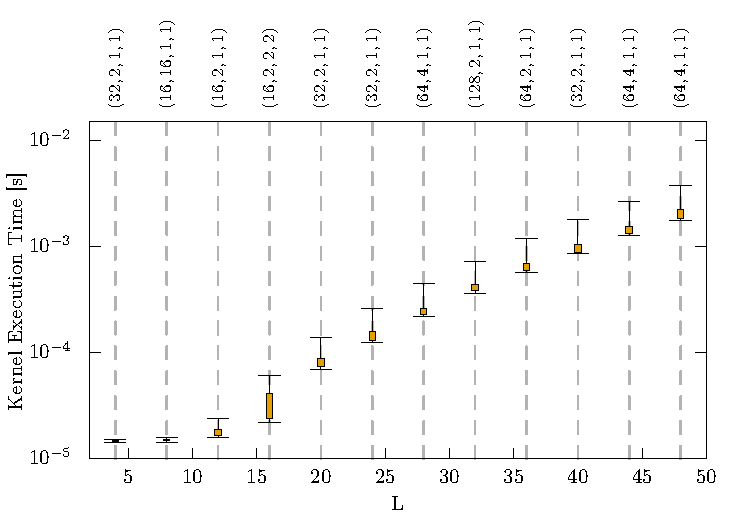
\includegraphics[width=\textwidth]{figs/tiling_distr_L_boxplot_v2.pdf}
  \end{columns}

\end{frame}

\begin{frame}{Benchmark: Linear algebra kernels}{cpu}

  \begin{itemize}
    \item Benchmark on a single node of the Juwels Booster
    \item AMD EPYC 7402 cpu, 48 threads, no SMT
    \item compiled with GCC 13.3
  \end{itemize}

  \begin{columns}
    \column{0.5\textwidth}
      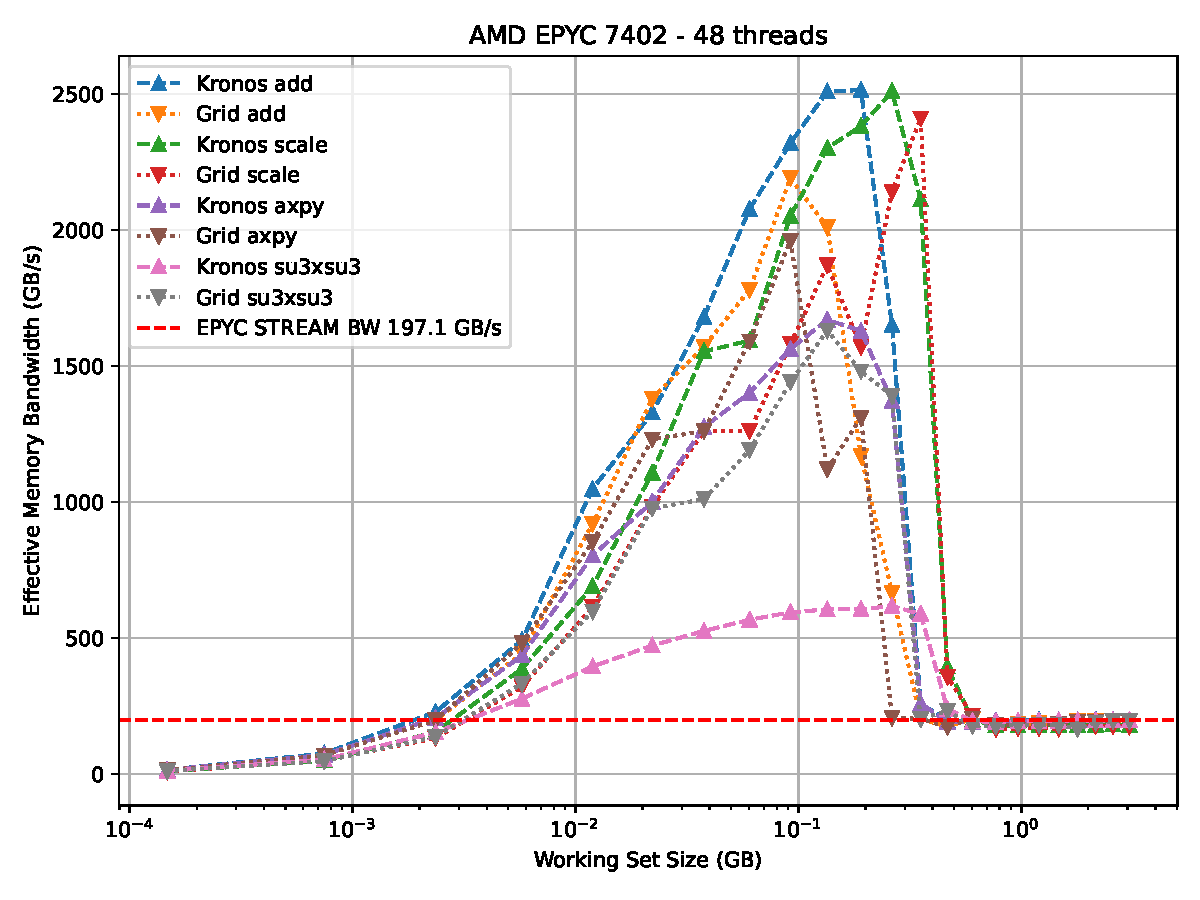
\includegraphics[width=\textwidth]{figs/comparison_grid_epyc.pdf}
    \column{0.5\textwidth}
      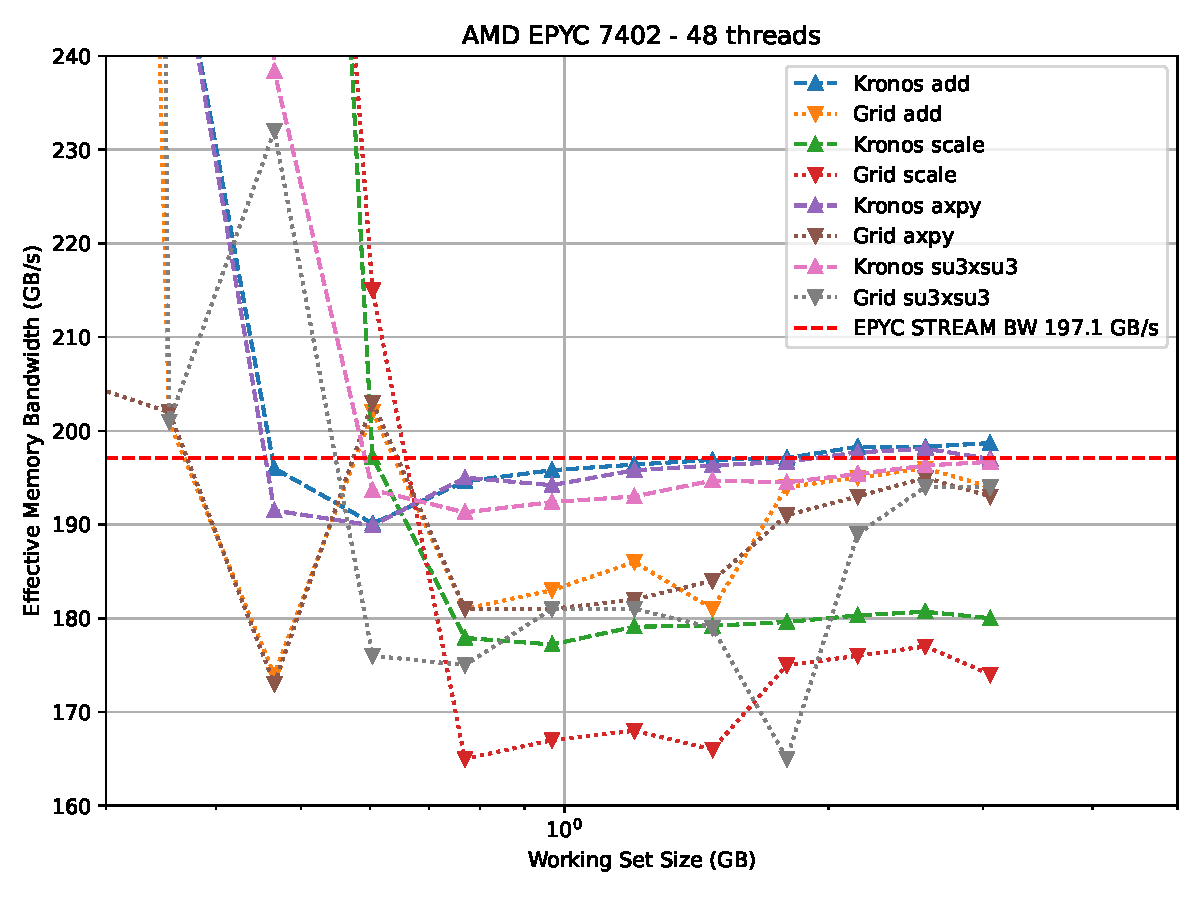
\includegraphics[width=\textwidth]{figs/comparison_grid_epyc_zoomed.pdf}
  \end{columns}
\end{frame}

\begin{frame}{Benchmark: Linear algebra kernels}{gpu}

  \begin{itemize}
    \item Benchmark on a single gpu in a single node of the Juwels Booster
    \item NVIDIA A100 40 GB
    \item compiled with NVCC 12.6
  \end{itemize}

  \begin{columns}
    \column{0.5\textwidth}
      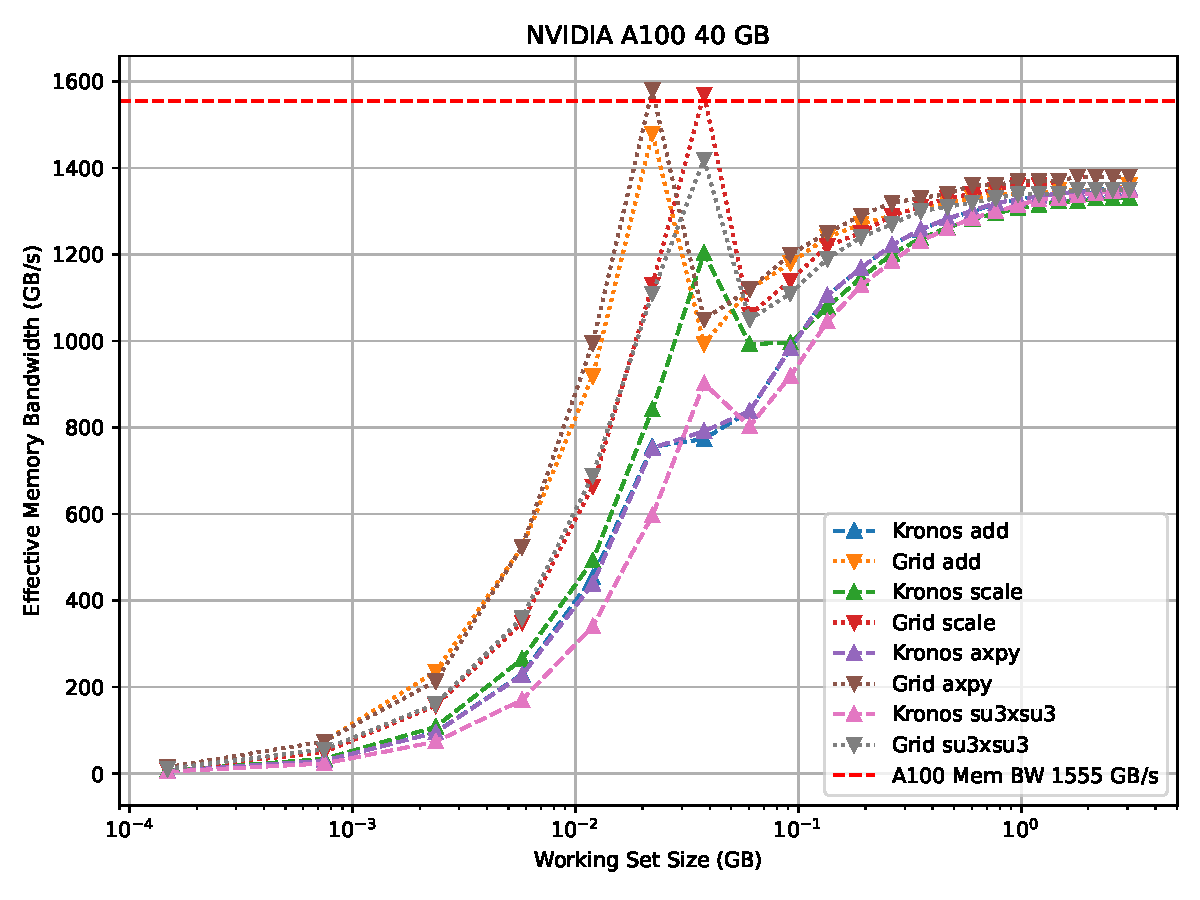
\includegraphics[width=\textwidth]{figs/comparison_grid_a100.pdf}
    \column{0.5\textwidth}
      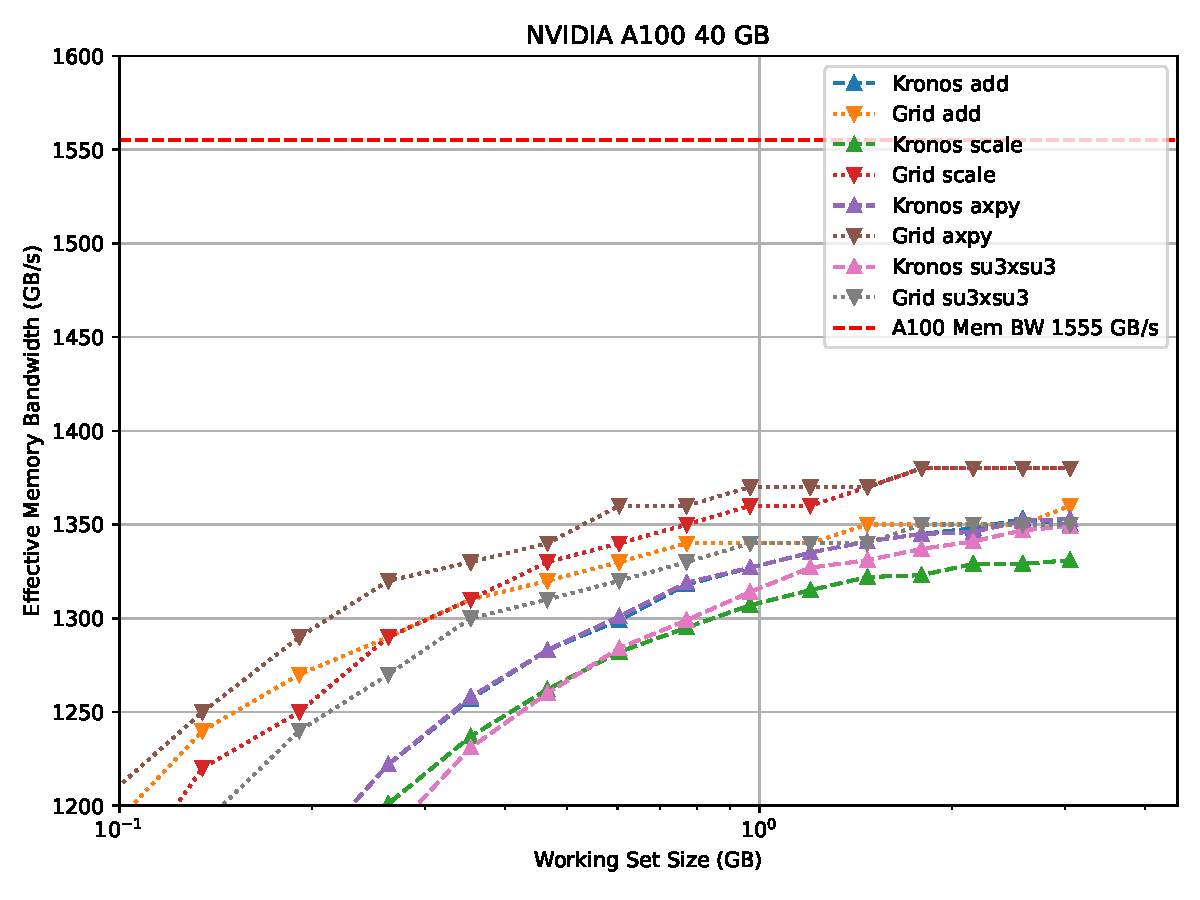
\includegraphics[width=\textwidth]{figs/comparison_grid_a100_zoomed.pdf}
  \end{columns}
\end{frame}

\begin{frame}{Towards Actual Physics}{current status}

  \begin{bkblock}{LEMON}
    \begin{itemize}
      \item a functional lemon interface to read and write gauges
    \end{itemize}
  \end{bkblock}

  \begin{bkalertblock}{QUDA}
    \begin{itemize}
      \item a working interface to QUDA
      \item transfer gauge and spinor fields between Kronos and QUDA
      \item gauge and propagator smearing
      \item a solver interface (only CGNE at the moment)
      \item Dslash interface to QUDA
    \end{itemize}
  \end{bkalertblock}

  \begin{bkexampleblock}{Dslash}
    \begin{itemize}
      \item a working Wilson Dslash implementation in Kronos (only M)
      \item crosschecked against QUDA for correctness
    \end{itemize}
  \end{bkexampleblock}

  \begin{bkblock}{Correlator}
    \begin{itemize}
      \item a simple meson 2 point correlator for different gamma matrices
    \end{itemize}
  \end{bkblock}

\end{frame}

\end{document}
